\begin{enumerate}[label=\thesection.\arabic*.,ref=\thesection.\theenumi]
\numberwithin{equation}{enumi}

\item
For a unity Feedback system 
\begin{align}
    G(s) = \frac{K}{s(s+2)(s+4)(s+6)}
\end{align}


Design a PD Controller with $K_{v} = 2$ and Phase Margin 30\degree

\solution
PD Controller is cascaded with the given G(s).
The Transfer Function of the PD Controller is $K_{p}(1 + T_{d}s)$

\begin{align}
    G_{c}(s) = \frac{K_{p}(1 + T_{d}s)K}{s(s+2)(s+4)(s+6)}
\end{align}

\begin{align}
    K_{v} = \lim_{s \to 0} sG_{1}(s) = 2
\end{align}

If we choose $K_{p} = 1$
\begin{align}
    \implies K = 96
\end{align}

For Phase Margin 30\degree, at Gain Crossover Frequency w

\begin{align}
    \tan^{-1}(T_{d}\omega) - \tan^{-1}(\frac{\omega}{2}) - \tan^{-1}(\frac{\omega}{4})
    \tan^{-1}(\frac{\omega}{6}) = -60
\end{align}

\begin{align}
    \abs{G_{1}\brak{\j\omega}} = \frac{96\sqrt{T_{d}^2w^2 + 1}}{w\sqrt{(w^2+4)(w^2 + 16)(w^2 + 36)}} = 1
\end{align}

Solving these equations is really complicated,
By Hit and Trial, one of the best combinations is
\begin{align}
    w = 4
\end{align}
\begin{align}
    T_{d} = 1.884
\end{align}
We get a Phase Margin of 30.31\degree

\item
Verify using a Python Plot

\solution
\begin{lstlisting}
codes/EE18BTECH11021_3.py
\end{lstlisting}

\begin{figure}
\centering
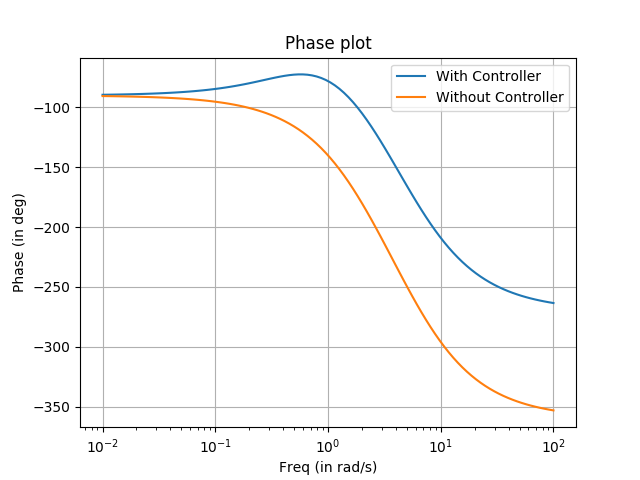
\includegraphics[width=\columnwidth]{figs/EE18BTECH11021_PD.png}
\end{figure}

\item
Design a PI Controller with $K_{v} = \infty$ and Phase Margin 30\degree

\solution
PI Controller is cascaded with the given G(s).
The Transfer Function of the PD Controller is $K_{p}(1 + \frac{1}{T_{i}s})$

\begin{align}
    G_{1}(s) = \frac{K_{p}(1 +  \frac{1}{T_{i}s})K}{s(s+2)(s+4)(s+6)}
\end{align}

Choose $K_{p}K = 96$
This can be written as
\begin{align}
    G_{1}(s) = \frac{96(T_{i}s + 1)}{T_{i}s^2(s+2)(s+4)(s+6)}
\end{align}

For Phase Margin 30\degree, at Gain Crossover Frequency w

\begin{align}
    \tan^{-1}(T_{i}\omega) - \tan^{-1}(\frac{\omega}{2}) - \tan^{-1}(\frac{\omega}{4})
    \tan^{-1}(\frac{\omega}{6}) = 30
\end{align}

\begin{align}
    \abs{G_{1}\brak{\j\omega}} = \frac{96\sqrt{T_{i}^2w^2 + 1}}{T_{i}^2w^2\sqrt{(w^2+4)(w^2 + 16)(w^2 + 36)}} = 1
\end{align}

By Hit and Trial, one of the best combinations is
\begin{align}
    w = 0.75
\end{align}
\begin{align}
    T_{i} = 2.713
\end{align}
We get a Phase Margin of 25.53\degree

\item
Verify using a Python Plot

\solution
\begin{lstlisting}
codes/EE18BTECH11021_4.py
\end{lstlisting}

\begin{figure}
\centering
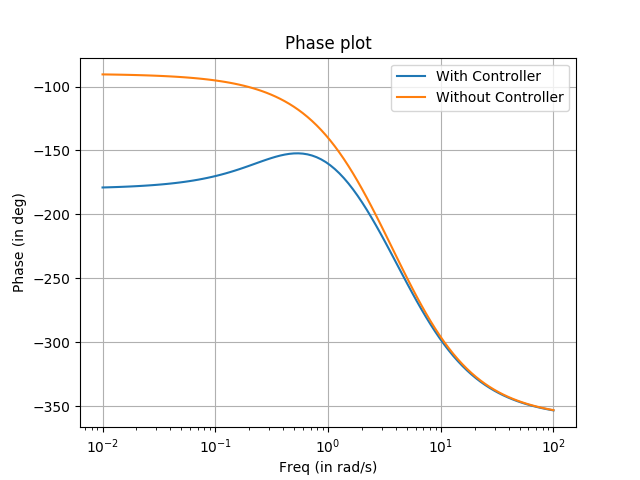
\includegraphics[width=\columnwidth]{figs/EE18BTECH11021_PI.png}
\end{figure}

\item
Design a PID Controller with $K_{v} = \infty$ and Phase Margin 30\degree

\solution
PID Controller is cascaded with the given G(s).
The Transfer Function of the PD Controller is $K_{p} + K_{d}s + \frac{K_{i}}{s}$

\begin{align}
    G_{1}(s) = \frac{(K_{p}+ K_{d}s + +\frac{K_{i}}{s})K}{s(s+2)(s+4)(s+6)}
\end{align}

Choose $K_{p}K = 96$
This can be written as
\begin{align}
    G_{1}(s) = \frac{96(T_{i}T_{d}s^2 + T_{i}s +  1)}{T_{i}s^2(s+2)(s+4)(s+6)}
\end{align}

For Phase Margin 30\degree, at Gain Crossover Frequency w

\begin{align}
    \tan^{-1}(\frac{T_{i}\omega}{1-T{i}T_{d}w^2}) - \tan^{-1}(\frac{\omega}{2}) - \tan^{-1}(\frac{\omega}{4})
    \tan^{-1}(\frac{\omega}{6}) = 30
\end{align}

\begin{align}
    \abs{G_{1}\brak{\j\omega}} = \frac{96\sqrt{(1-T{i}T_{d}w^2)^2 + T_{i}^2}}{T_{i}^2w^2\sqrt{(w^2+4)(w^2 + 16)(w^2 + 36)}} = 1
\end{align}

By Hit and Trial, one of the best combinations is
\begin{align}
    w = 1
\end{align}
\begin{align}
    T_{i} = 1.738
\end{align}
\begin{align}
    T_{d} = 0.4
\end{align}
We get a Phase Margin of 30\degree

\item
Verify using a Python Plot

\solution
\begin{lstlisting}
codes/EE18BTECH11021_5.py
\end{lstlisting}

\begin{figure}
\centering
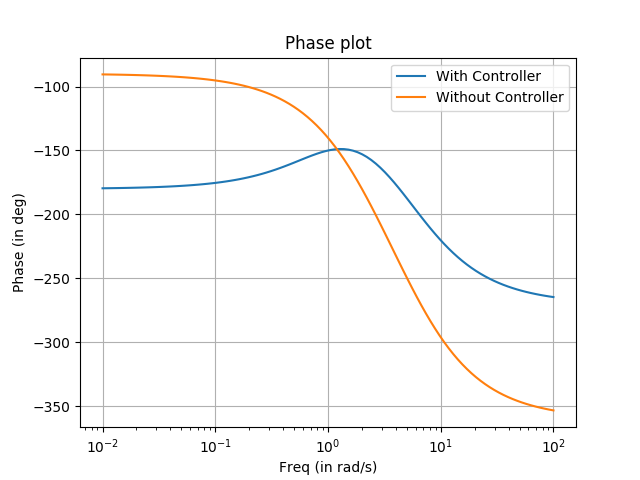
\includegraphics[width=\columnwidth]{figs/EE18BTECH11021_PID.png}
\end{figure}